\documentclass{article}
\usepackage{homework}
\usepackage{multirow}
\usepackage{tikz}
\usetikzlibrary{positioning}
\usetikzlibrary{arrows}
% \usepackage[ruled, vlined]{algorithm2e} % 算法与伪代码
\usepackage{algorithm}
\usepackage{algpseudocode}
\bibliographystyle{ieeetr}

\title{Baseline is All You Need: the Story of Us Failing to Outperform Project Baselines}
\author{时若曦-519030910373 \quad 杨博睿-519030910374}
\date{}

\begin{document}
\maketitle

% Introduction
\section{Introduction}\label{sec:Intro}


% Related Work
\section{Related Work}\label{sec:RelatedWork}
    \subsection{Attacks}


    \subsection{Defenses}
    To cope with security risks posed by adversarial examples, many novel defensive methods have been proposed, including adversarial training, hypersphere embedding \cite{pang2020boosting} and gradient obfuscation. (However, gradient obfuscation proves to be vulnerable under specifically-designed attacks \cite{athalye2018obfuscated}.)

    We detail two related major techniques in adversarial defense.
    \paragraph{TRADES.} TRADES \cite{zhang2019theoretically} modifies the cross-entropy loss in adversarial training to achieve a trade-off between accuracy and model robustness.
    \begin{equation}\label{eq:trades}
        \min_{\mathbf{w}} \frac{1}{n}\sum_{i=1}^n \left( \mathcal{L}_{CE}\left( f_{\mathbf{w}}(\mathbf{x}_i), y_i \right) + \gamma\mathcal{L}_{KL}\left(f_{\mathbf{w}}(\mathbf{x}_i), f_{\mathbf{w}}(\mathbf{x}_i^{adv})\right) \right)
    \end{equation}
    where $\mathbf{x}^{adv}$ is the adversarial example, $\mathcal{L}_{CE}(\cdot)$ and $\mathcal{L}_{KL}(\cdot)$ are cross-entropy loss and Kullback-Liebler Divergence, repectively.

    \paragraph{Adversarial Weight Perturbation.} Adversarial Weight Perturbation (AWP) \cite{wu2020adversarial} aims to narrow the robust generalization gap of AT models. It flattens the ``weight-loss landscape'' by adding extra perturbations to model parameters during adversarial training. This is based on an observation that models with good performance on unforeseen test data tend to have flatter weight-loss landscape. AWP solves the optimization problem in (\ref{eq:awp}).
    \begin{equation}\label{eq:awp}
        \min_{\mathbf{w}} \max_{\mathbf{v} \in \mathcal{V}} \frac{1}{n}\sum_{i=1}^n \max_{\|\mathbf{x}^{adv} - \mathbf{x}\|_p \le \epsilon} \mathcal{L}(f_{\mathbf{f}+\mathbf{v}}(\mathbf{x}^{adv}_i), y_i)
    \end{equation}
    where $l(\cdot)$ is a loss function, $\mathbf{v}$ is the perturbation in model weight and $\mathcal{V}$ is the feasible region of weight perturbation.


% Attack
\section{The Frank-Wolfe AdAmp Attack}\label{sec:FWAdAmpAttack}
    \subsection{Frank-Wolfe: A Parameter-free Attack}
        The Frank-Wolfe algorithm \cite{frank1956algorithm} is a well known algorithm for constrained convex optimization with first order (gradient) information. It is also known as the convex combination algorithm.
        
        For the sake of briefness, the general form of the algorithm is not presented. Rather, we directly demonstrate here the version adapted for adversarial attack in $L_\infty$-norm.
        
        \begin{algorithm}[h]
            \caption{Frank-Wolfe Parameter-free Attack}
            \label{alg:FWPFA}
            \hspace*{\algorithmicindent} \textbf{Input}: model $M$, target input $x$, ground truth label $y_t$, $L_\infty$-norm bound $\epsilon$, steps limit $s$ \\
            \hspace*{\algorithmicindent} \textbf{Output}: perturbation $\Delta$
            \begin{algorithmic}[1]
                \State $\Delta \leftarrow \mathbf{0}$ 
                \For {$k = 0 \dots s - 1$}
                    \State $g^\star \leftarrow \epsilon \cdot \mathrm{sgn}\left(\nabla \mathcal{L}(M(x + \Delta), y_t)\right)$
                    \State $\alpha \leftarrow \frac{2}{k + 2}$
                    \State $\Delta \leftarrow \alpha \cdot g^\star + (1 - \alpha)\cdot\Delta$
                \EndFor
            \end{algorithmic}
        \end{algorithm}
        
        The algorithm tries to maximize a loss function $\mathcal{L}$ between classifier output and ground truth (For the loss we adopted see Sec.\ \ref{sub:AdAmp}). In each step, we approximate the loss with a linear function via gradient information at current perturbed input, and solve for the optima $g^\star$ within the $L_\infty$ norm bound in the resulting approximation (line 3). A decaying combination factor $\alpha$ is computed (line 4) and the perturbation is updated with a convex combination between $g^\star$ and the result at the previous step (line 5).
        
        For any convex target constrained on a convex compact set, the convergence rate is guaranteed to be at least $O(1/k)$, where $k$ is number of steps performed, according to primal-dual analysis presented in \cite{jaggi2013revisiting}. The attack provides in general a good amount of attack strength without the need of intensively adjusting the parameters, such as step size of the PGD attack.
    

    \subsection{Adaptive Amplification} \label{sub:AdAmp}
        Cross-entropy measures the distributional distance between model prediction and ground truth. It is suitable as a loss for classification task, and is widely adopted in the training process of artificial neural networks.
        
        On the other hand, regular softmax cross-entropy does not necessarily reflect well on the success of classification, especially in the case where top-k classes have similar predicted logits. This case is quite common during iterations of adversaries.
        
        We thus proposed Adaptive Amplification. It is applied to obtain a better target function in place of the regular softmax cross-entropy for adversarial attacks.
        
        \paragraph{Amplifying the Difference} The softmax distribution is invariant upon additive constants. Thus, only the relative difference between the pre-activation logits affects the distribution ($\Delta$ is used to indicate the invariance). We consider amplifying the difference: instead of
        \newcommand{\vdz}{\Delta \mathbf{z}}
        \begin{equation}
            \sigma(\vdz)_i = \frac{e^{\vdz_i}}{\sum e^{\vdz}_j},
        \end{equation}
        we consider pre-multiplying by a factor of $w$
        \begin{equation}
            \sigma_w(\vdz)_i = \frac{e^{w\vdz_i}}{\sum e^{w\vdz_j}}.
        \end{equation}
        When $w > 1$ this greatly amplifies the difference between classes. Since we the target is to find wrongly classified examples through gradient, the closer the target loss geometry is to the `hard' classification decision boundary the better information the gradient will provide us. The amplification procedure thus makes finding adversarial examples close to the decision boundary easier (See Fig.\ \ref{fig:softmax_preamp}).
        
        \begin{figure}[ht]
            \centering
            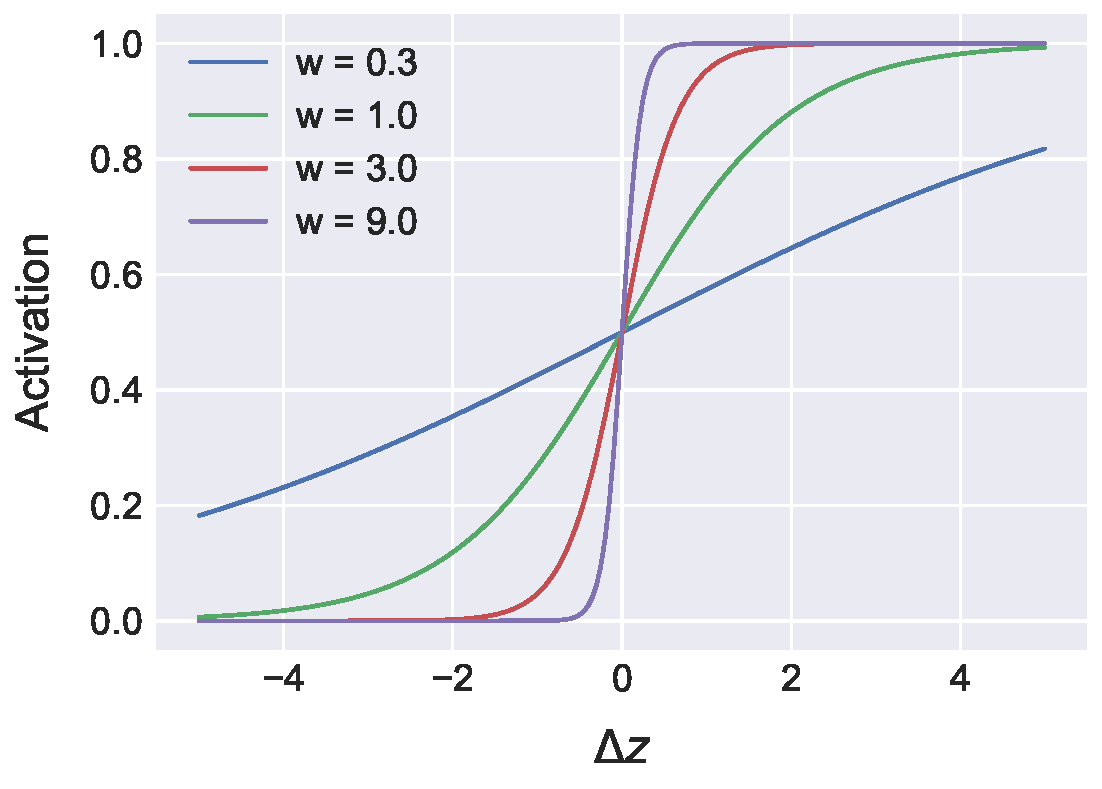
\includegraphics[width=0.5\linewidth]{figs/bin_amp_geo.pdf}
            \caption{\textbf{Geometry of binary softmax cross-entropy after amplification.} Application of different amplification factors $w$ on binary softmax cross-entropy are shown. It can be seen that large $w$'s significantly amplify difference between classes. $w = 1$ means regular softmax cross-entropy.}
            \label{fig:softmax_preamp}
        \end{figure}
        
        \paragraph{Adaptive Amplification} Theoretically, an amplification factor $w \to +\infty$ is best suited for the application since the target function approaches classification correctness at the limit. However, the gradient may numerically vanish if $\vdz$ is amplified to a large value. So we need to choose $w$ carefully. Conversely, if the original model outputs a large $\vdz$ which cause the gradient to vanish for a regular cross-entropy, we may be willing to apply a $w < 1$ to let useful gradient information in.
        
        Since differentiation is a linear operator, we may sum up values at different $w$'s. Since we are still willing to approximate the classification correctness as well as we can do, we give larger weights to larger $w$'s. The final loss function is
        \begin{equation}
            \mathcal{L}(\vdz) = \sum_{w \in W} w^2 H(\sigma_w(\vdz), y_t),
        \end{equation}
        where $\vdz$ is the logits before activation, $H$ is cross-entropy function and $y_t$ is ground truth distribution. $W$ is a pre-defined list of possible amplification factors that typically span several orders of magnitude. In the experiments we take $W = [0.3, 1, 2, 3, 4, 5, 6, 7, 8, 9, 10]$.
        
        Note that the forward and backward passes of the entire model only needs to be performed once for the proposed target loss. There is almost no extra computational cost for Adaptive Amplification.


% Defense
\section{Frank-Wolfe-based Defense}\label{sec:DefenseMethodology}
    In this section, we detail our design of adversarial defense. Since we fail to come up with fancy innovative defense ideas that works properly, we fallback to traditional adversarial training approaches, and integrate our proposed FW-AdAmp attack method with various adversarial training methods.

    \subsection{Frank-Wolfe Defense}
        We utilize the FW-AdAmp method and improve adversarial training by substituting FW-AdAmp attack for standard PGD attacks in adversarial trainings. Let $\mathbf{x}^{adv}$ denote the adversarial example generated by FW-AdAmp, we then train a robust model by solving the optimization in (\ref{eq:fwat}).
        \begin{equation}\label{eq:fwat}
            \min_{\mathbf{w}} \frac{1}{n}\sum_{i=1}^n \mathcal{L}_{CE}(f_{\mathbf{w}}(\mathbf{x}^{adv}_i), y_i))
        \end{equation}

    \subsection{Combination with Other AT Methods}
        FW-AdAmp attack can also be flexibly combined with other AT methods. In this section, we introduce the combination of FW-AdAmp method with AWP and TRADES.

        \paragraph{Combination with TRADES.} The combination with TRADES is also straightforward: it can be done by simply changing the loss from cross-entropy to TRADES loss given in (\ref{eq:trades}).

        \paragraph{Combination with Adversarial Weight Perturbation.} The role of FW-AdAmp attack is similar to that of a PGD attack in the AT-AWP framework proposed by Wu et al. Therefore to combine FW-AdAmp with AWP, we simply change the attack method from PGD to FW-AdAmp in the AT-AWP framework.


% Experiments and Results
\section{Results}\label{sec:Results}
    \subsection{Attack}\label{sub:AttackExp}
    \begin{table}[h]
        \centering
        \begin{tabular}{cccccccc}
            \hline
            Method         & M1            & M2             & M3             & M4             & M5             & M6             & BWD/FWD       \\ \hline
            No attack      & 94.29         & 83.02          & 80.33          & 84.92          & 81.43          & 88.25          & -             \\
            PGD20          & 0.04          & 51.29          & 65.15          & 56.18          & 54.82          & 64.34          & \textbf{20/0} \\
            DeepFool       & 0.02          & 48.05          & 31.60          & 53.81          & 52.55          & 60.99          & 200/20        \\
            Sobol Sampling & 75.30         & 79.96          & 60.52          & 82.33          & U              & U              & 0/200         \\
            Chihao Happy   & 63.53         & 79.59          & 42.26          & U              & U              & U              & 0/200         \\
            ReLeak-PGD     & 5.36          & U              & \textbf{19.97} & 83.20          & U              & 86.80          & \textbf{20/0} \\
            Krylov         & U             & U              & U              & 56.03          & U              & 65.10          & 20/20         \\
            F-W            & \textbf{0.00} & 50.25          & 63.12          & 55.30          & 53.46          & 63.79          & \textbf{20/0} \\
            F-W-Amp        & 60.32         & 48.11          & 56.34          & 53.50          & 53.00          & 60.92          & \textbf{20/0} \\
            F-W-AdAmp      & \textbf{0.00} & \textbf{47.79} & 45.00          & \textbf{53.27} & \textbf{52.35} & \textbf{60.54} & \textbf{20/0} \\ \hline
            \end{tabular}
        \caption{Results of 6 baseline models, under various attack attempts.}
    \end{table}
    \begin{figure}[H]
        \centering
        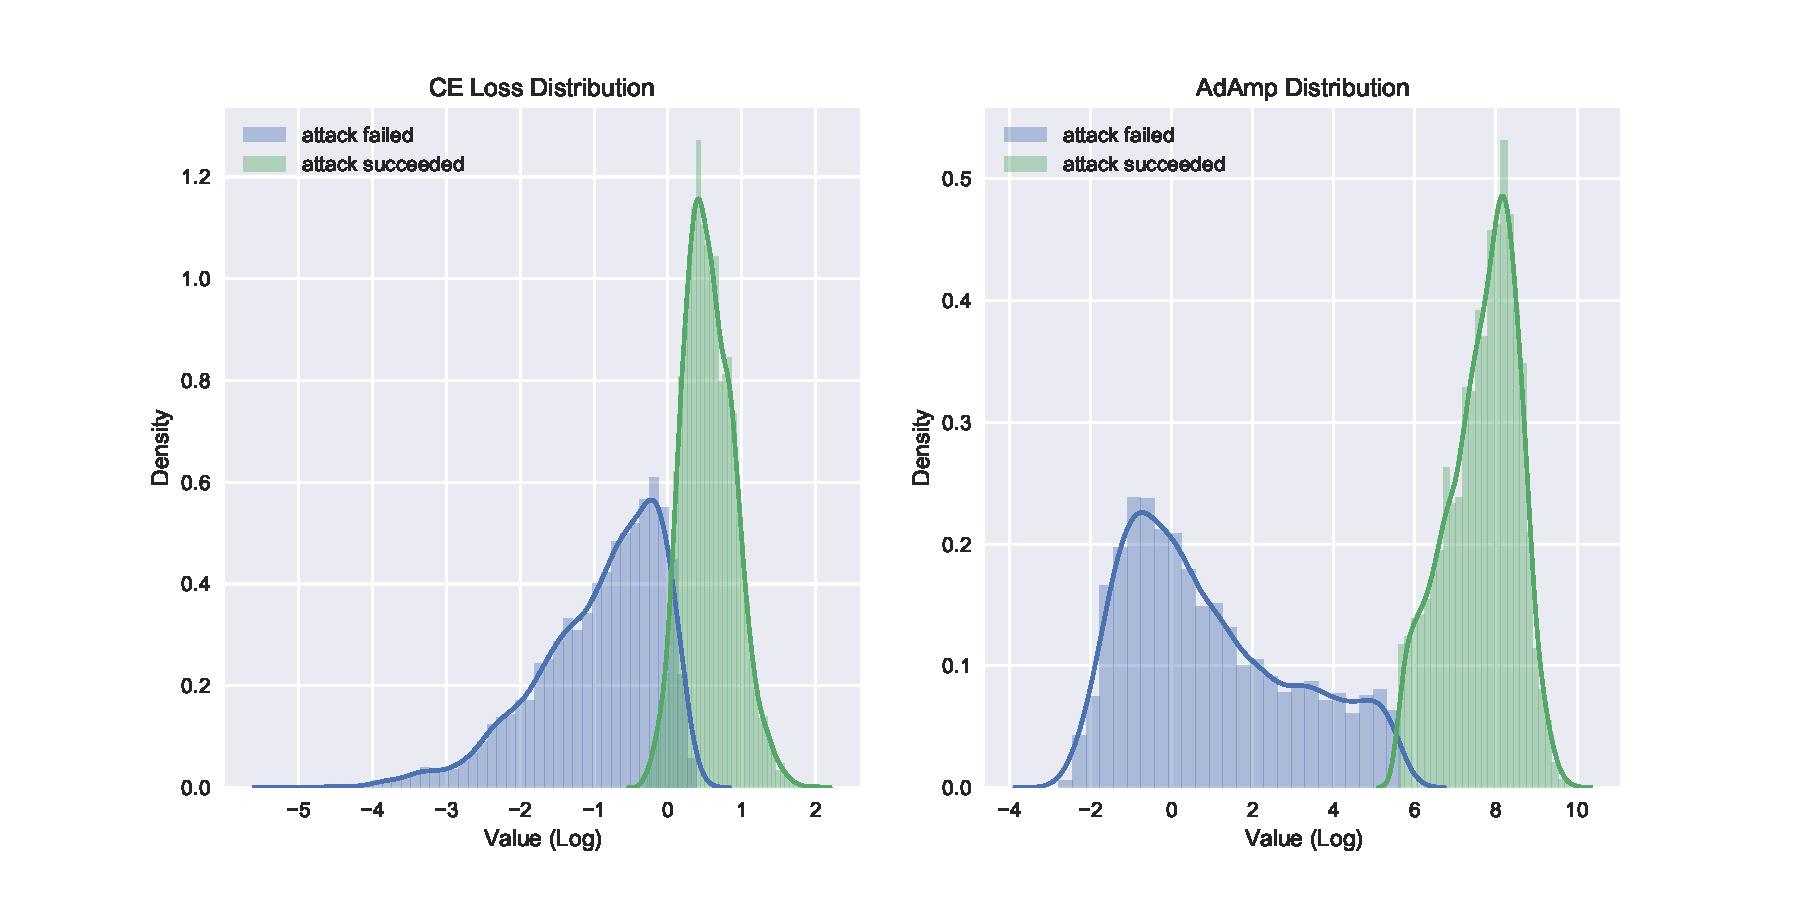
\includegraphics[width=0.9\textwidth]{figs/ce_adamp_distribution.pdf}
        \caption{Placeholder}
        \label{fig:loss_distribution}
    \end{figure}
    \subsection{Defense}\label{sub:DefenseExp}
        In this section, we present the experiment results on our defense models.
        \subsubsection{Experiment Setup}\label{subs:DefenseExpSetup}
             All defense models are trained for 100 epochs, using SGD optimizer with momentum 0.9 and weight decay $5\times 10^{-4}$. We set the learning rate to 0.1, which is mutiplied by 0.1 at 75th and 90th epoch. For Adversarial Weight Perturbation, we set the parameter $\gamma$ to be $0.1$ and set a warm up of 10 epochs. For TRADES loss, we set the hyperparameter $\beta = 1/\lambda = 6.0$.

            All models are trained on 2 NVIDIA GTX 1080Ti GPUs.

        \subsubsection{Benchmarking on Different Models}\label{subs:DefenseModelBenchmarking}
            \begin{table}[h]
                \centering
                \begin{tabular}{cccccc}
                    \hline
                    Models                         & Loss                        & Time      & Natural        & PGD20          & FW-AdAmp             \\ \hline
                    \multirow{3}{*}{ResNet18}      & \multicolumn{1}{l}{AT(PGD)} & -         & 83.57          & 51.38          & 48.13          \\
                                                   & AT(FW)                      & 6.06 hrs  & 79.48          & 55.88          & 49.98          \\
                                                   & TRADES                      & 7.01 hrs  & 78.35          & 55.93          & 49.04          \\ \hline
                    \multirow{2}{*}{Wide ResNet28} & AT(FW)                      & 25.61 hrs & \textbf{84.75} & 59.39          & \textbf{55.34} \\
                                                   & TRADES                      & 29.82 hrs & 82.17          & \textbf{60.02} & 53.65          \\ \hline
                    ResNet34                       & AT(FW)                      & 10.38 hrs & 81.74          & 57.99          & 52.91          \\ \hline
                    PreAct ResNet18                & AT(FW)                      & 5.92 hrs  & 80.41          & 55.76          & 50.14          \\ \hline
                    PreAct ResNet34                & AT(FW)                      & 10.34 hrs & 81.86          & 57.90          & 53.80          \\ \hline
                \end{tabular}
                \caption{Benchmarking different models. Except the baseline, all models are trained with FW-AdAmp w/ AWP. We use PGD and FW-AdAmp, both with 20 perturbation steps, to test robustness. Evaluation is run on the test set of CIFAR-10. Models use weights of their \emph{best} epoch.}
                \label{table:DefenseBenchmarkingResults}
            \end{table}

            We train several models using FW-AdAmp w/ AWP to evaluate our defense method. We use a PGD-10 AT ResNet-18 model as our baseline. The PGD used in AT has a step size of 0.007 and perturbation steps of 10. 

            Table \ref{table:DefenseBenchmarkingResults} reports the total training time and accuracy of different models, under both PGD attack and FW-AdAmp attack.

            The best robust accuracy under PGD20 (60.02\%) is achieved by Wide ResNet-28, trained with FW-AdAmp w/ AWP and TRADES loss. Notice that although we use identical network architecture and similar training framework, our model is still less robust than model 6, which achives a robust accuracy of 64.34\% under PGD20. This may because model 6 uses RST pretrain and 200 training epochs.

            To evaluate the combination of FW-AdAmp and TRADES loss, we also train ResNet-18 and Wide ResNet-28 using TRADES loss. Results suggest that TRADES loss can also bring extra improvements to model robustness.

            For a detailed comparision with ResNet-18 AT baseline, see Section \ref{subs:DefenseAgainstBaseline}
        
        \subsubsection{Comparision with Baseline}\label{subs:DefenseAgainstBaseline}
            \begin{table}[h]
                \centering
                \begin{tabular}{cccc}
                \hline
                AT Method          & Fwd & Bwd & Tot.Time \\ \hline
                PGD                & 0   & 10  & \textbf{5.55 hrs} \\
                FW-AdAmp           & 0   & 10  & 6.06 hrs \\
                FW-AdAmp w/ TRADES & 0   & 10  & 7.01 hrs \\ \hline
                \end{tabular}
                \caption{Training time of ResNet-18 model using the baseline PGD10, FW-AdAmp and FW-AdAmp w/ TRADES loss respectively. Adversarial training all use pertrubation step of 10.}
                \label{table:RN18TrnTime}
            \end{table}

            Using the same ResNet-18 network architecture, FW-AdAmp training (with AWP) improves robust accuracy under both attacks. The PGD10 baseline has an accuracy of 51.27\% under PGD20. Compared with the baseline, FW-AdAmp adversarial training boosts model robustness by about 4\% under PGD20 attack, and it also improves robustness under FW-AdAmp attack.
            
            Meanwhile, as is shown in Table \ref{table:RN18TrnTime}, FW-AdAmp has the same number of forward and backward propagation time with standard PGD 10. Dispite the extra time overhead caused mainly by the adaptive amplification when computing loss, the total training time using FW-AdAmp is similar to the training time of standard PGD 10 AT.
            
            These results demonstrate the advantage of FW-AdAmp for adversarial training.

        \subsubsection{Ablation Study on Wide ResNet-28}
            \begin{table}[h]
                \centering
                \begin{tabular}{ccccc}
                \hline
                AT Method          & Tot. Time          & Natural        & PGD20          & FW-AdAmp       \\ \hline
                TRADES-AWP         & 29.72 hrs          & 84.04          & 58.76          & 54.48          \\
                FW-AdAmp           & \textbf{25.61 hrs} & \textbf{84.75} & 59.39          & \textbf{55.34} \\
                FW-AdAmp w/ TRADES & 29.82 hrs          & 82.17          & \textbf{60.02} & 53.65          \\ \hline
                \end{tabular}
                \label{table:WRN28Ablation}
                \caption{Ablation study result of 3 Wide ResNet-28 models, trained with TRADES-AWP \cite{wu2020adversarial}, FW-AdAmp w/ AWP and FW-AdAmp w/ AWP and TRADES loss respectively.}
            \end{table}
            
            We further train a Wide ResNet-28 model using the TRADES-AWP method proposed by Wu et al. \cite{wu2020adversarial}. This model is trained for 100 epochs with PGD 10, using a SGD optimizer, AWP and TRADES with the same configuration.

            Table \ref{table:WRN28Ablation} reports the training time, natural and robust accuracies. FW-AdAmp with AWP and TRADES performs better than TRADES-AWP in terms of robust accuracy 


% Conclusion
\section{Conclusion}\label{sec:Conclusion}
We sugguest using model 6.


% Bibliography
\newpage
{\small
\bibliography{refs}
}

\end{document}